\documentclass{beamer}
\usetheme{Warsaw}

\setbeamertemplate{caption}[numbered]
\usepackage{copyrightbox}

\usepackage{siunitx}
\DeclareSIUnit\solarmass{\ensuremath{M_\odot}}

\title{Predicting the limits of the ELT}
\subtitle{Defensio}
\author[Alarich Herzner]{Alarich Herzner\\[1ex]  {\small Supervisor: Univ.-Prof. Jo\~ao Alves, PhD \\ Co-Supervisor: Dr. Kieran Leschinski, MSc}}
\institute{University of Vienna, Faculty of Physics}
\date{\today}

\begin{document}
\begin{frame}
\titlepage
\end{frame}

\begin{frame}
\frametitle{Outline}
\tableofcontents
\end{frame}

\section{Introduction}
\subsection{Goals}

\begin{frame}
\frametitle{Goals}
\begin{block}{Primary objective}
Estimate reliability limit for future IMF studies in the galactic centre using the ELT!
\end{block}
... what?
%\vspace{0.5cm}
\end{frame}

\begin{frame}
\frametitle{ELT}
  \begin{figure}
  \copyrightbox[b]{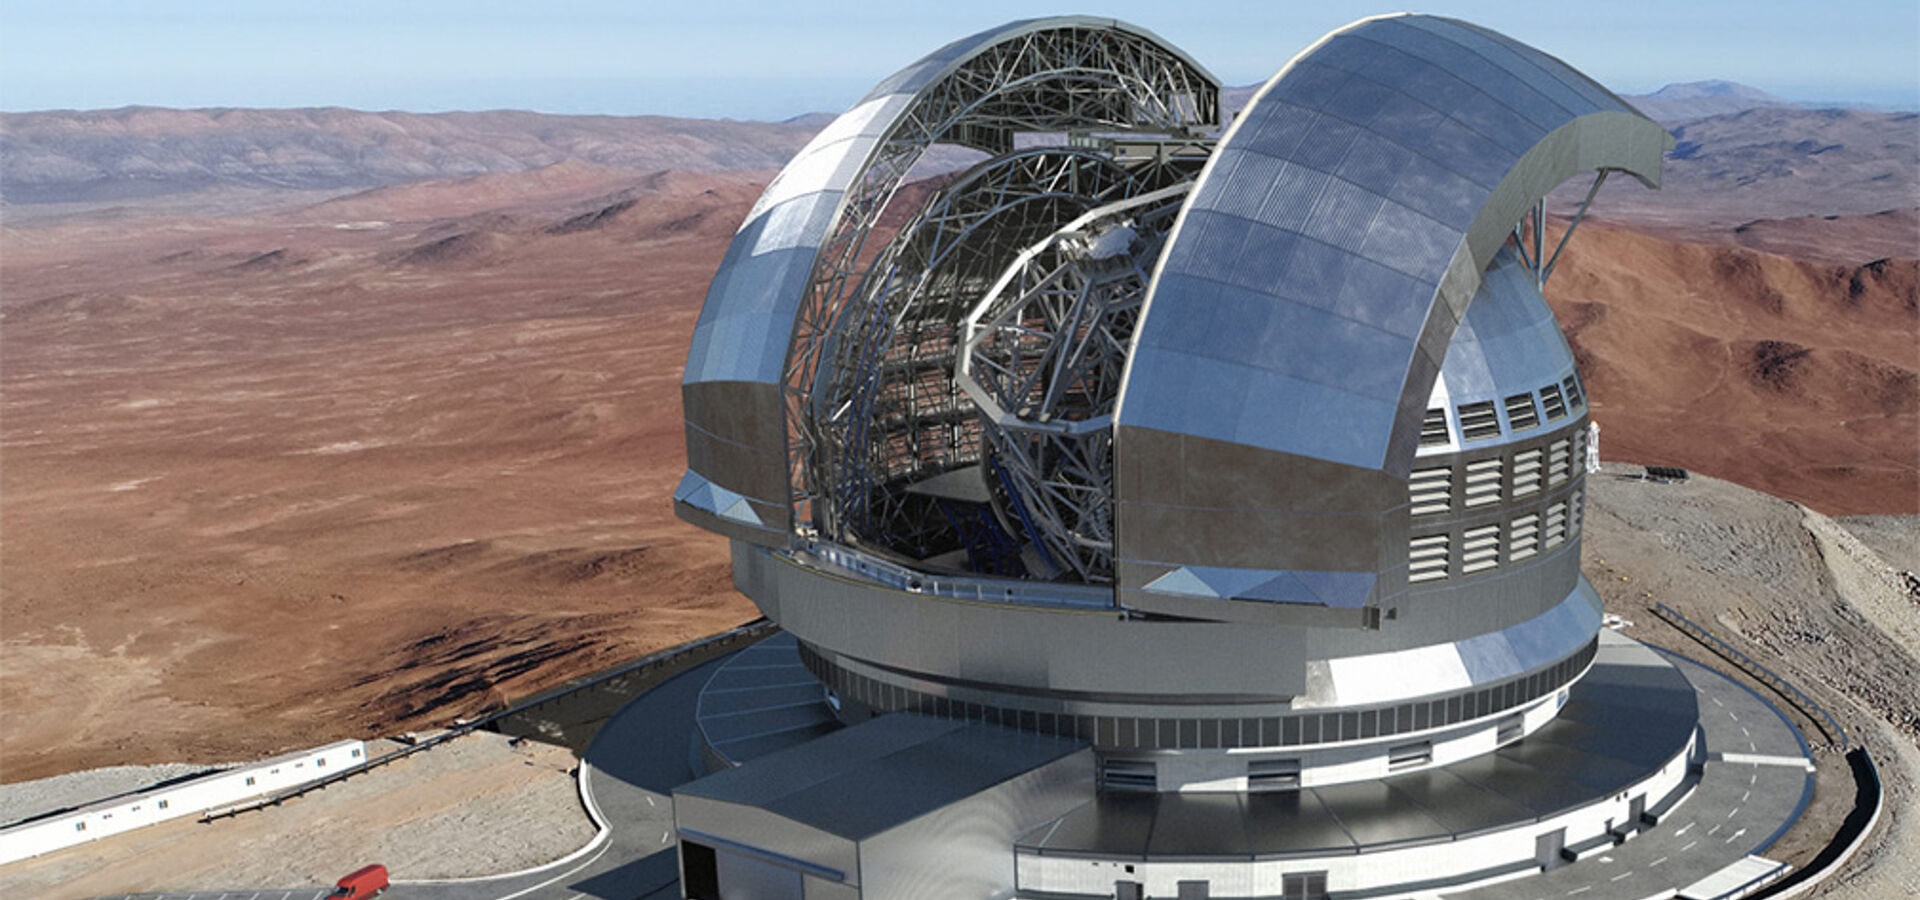
\includegraphics[width=\linewidth]{Images/ELT.jpg}}
                  {https://cdn.eso.org/images/banner1920/telescope-dome-landing.jpg}
  \end{figure}
\end{frame}

\begin{frame}
\frametitle{IMF}
  \begin{figure}
  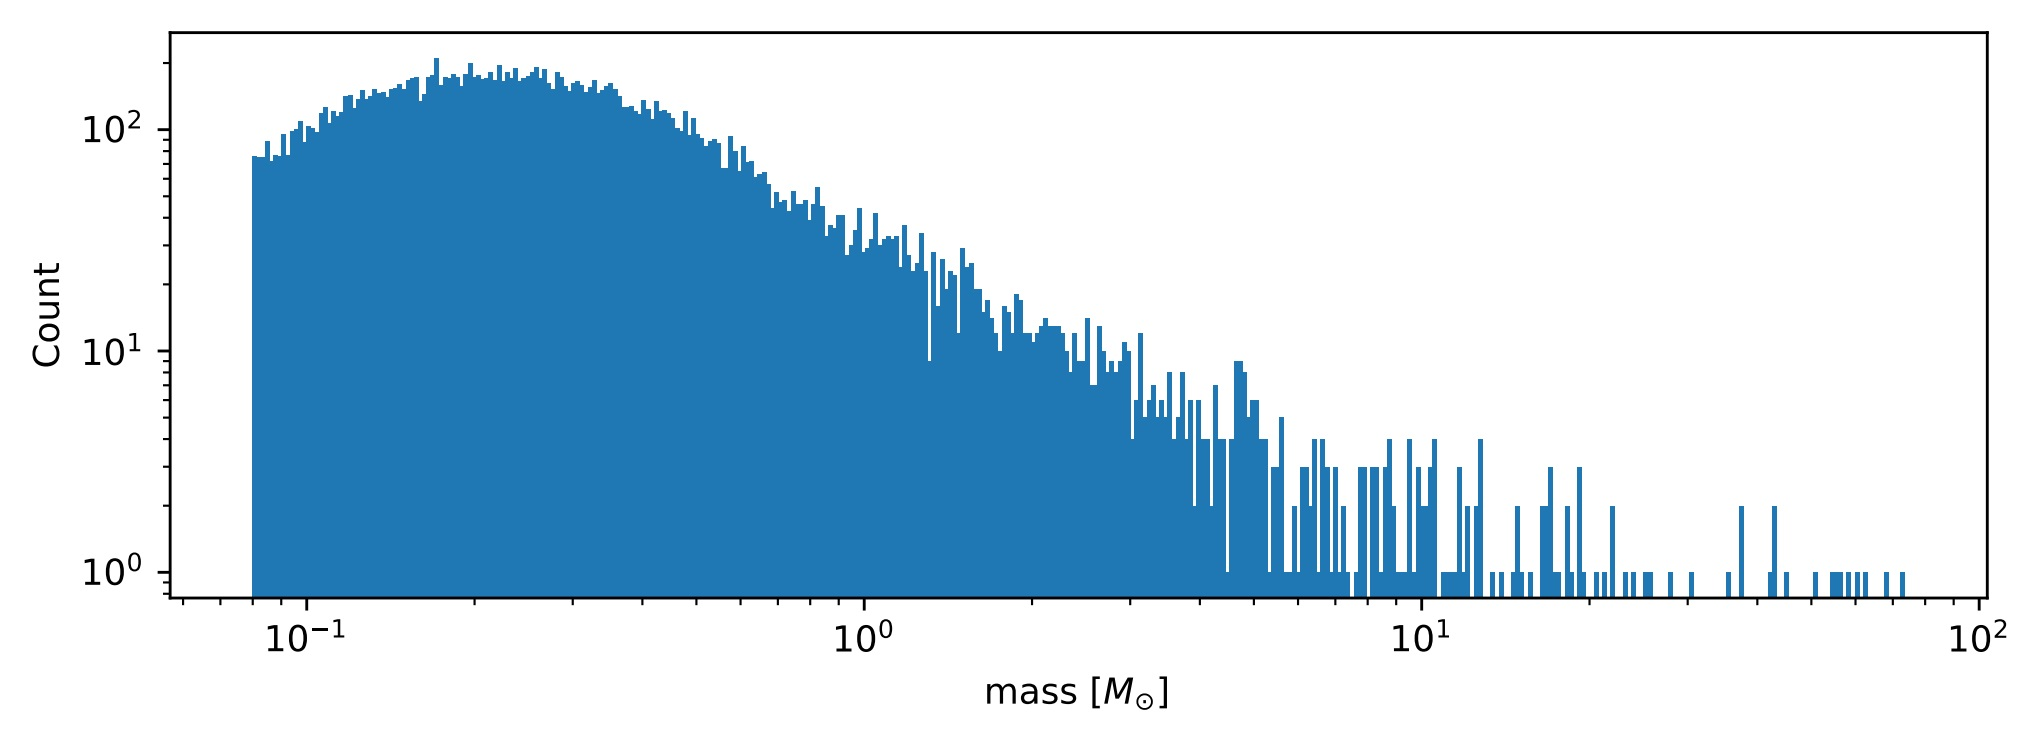
\includegraphics[width=\linewidth]{Images/IMF1.jpg}
  \end{figure}
\end{frame}

\begin{frame}
\frametitle{Reliability Limit}
  \begin{figure}
  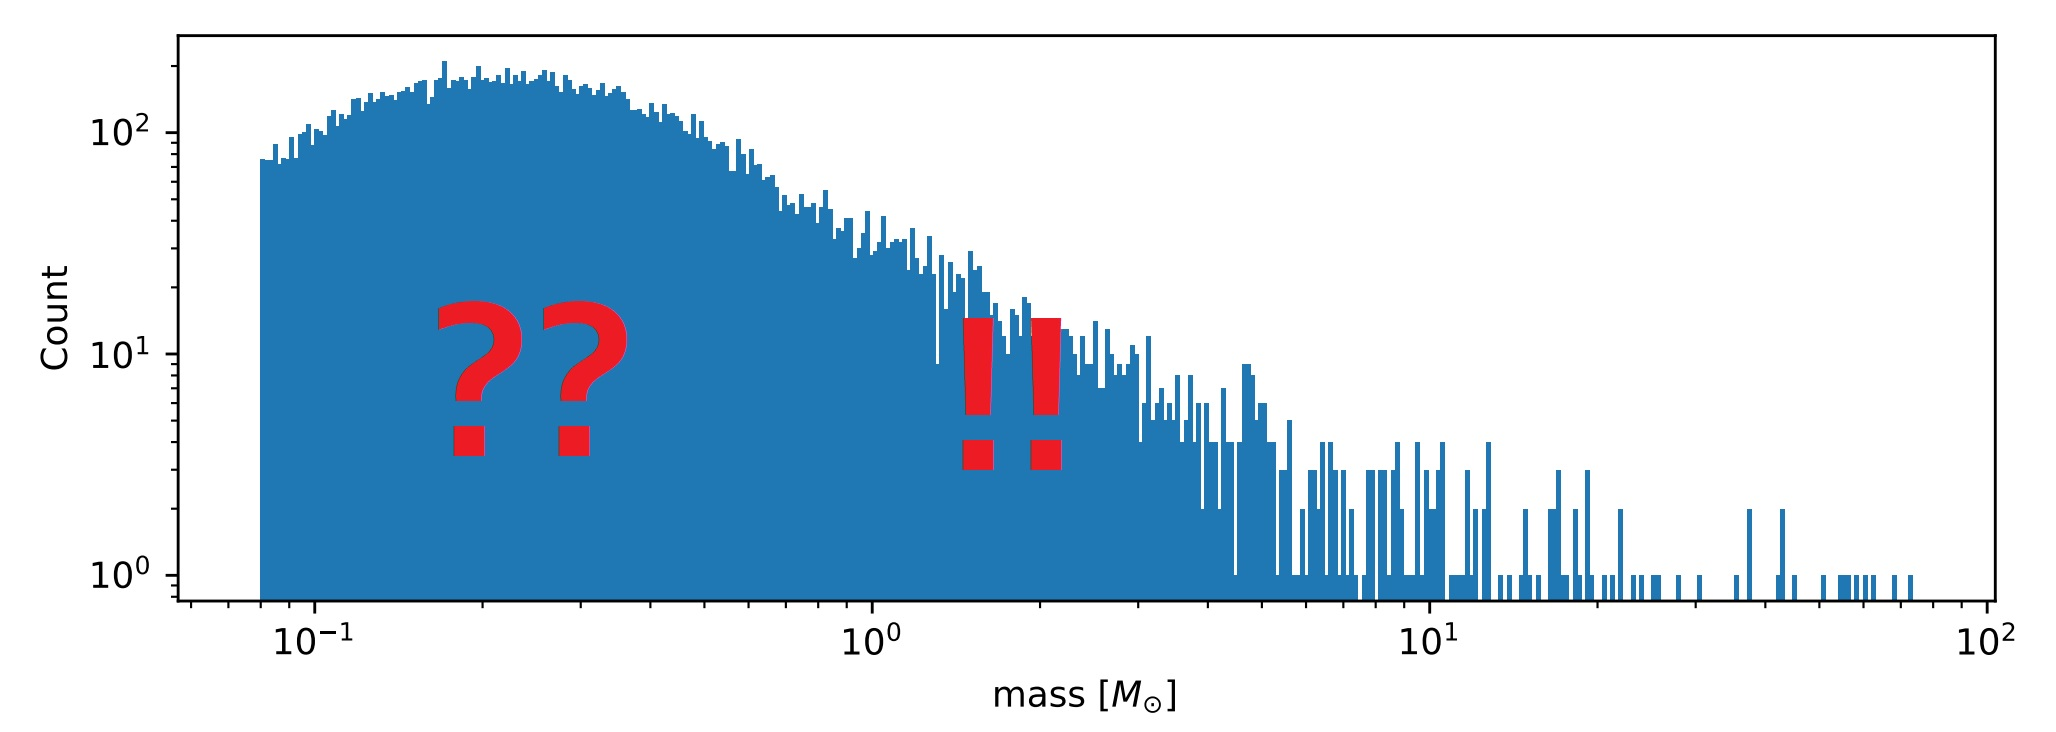
\includegraphics[width=\linewidth]{Images/IMF2.jpg}
  \end{figure}
\end{frame}

\subsection{Motivation}

\begin{frame}
\begin{block}{Motivation}
	\begin{columns}[T]
	\column{0.48\textwidth}
	\vspace{0.5em}
	\begin{itemize}
	\item Universal IMF?
	\item estimate number of lower-mass stars
	\item understand star formation process
	\end{itemize}
	\column{0.48\textwidth}
	\vspace{0.5em}
	\begin{itemize}
	\item N-body simulation with \(N \gg 1\)
	\item Clustering of time-dependent data
	\end{itemize}
	\end{columns}
\end{block}
\end{frame}


\subsection{Action Plan}

\begin{frame}
\frametitle{Action Plan}
\begin{enumerate}[I]
\item Simulate stars
\item Observe stars
\item Analyze
\item Measure performance
\end{enumerate}
\end{frame}

\section{Simulation}

\subsection{Cluster}

\begin{frame}
\frametitle{Parameters}
using McLuster

\begin{itemize}
\item Plummer density profile
\item virial equilibrium
\item Kroupa IMF \SIrange{0.08}{100}{\solarmass}
\item Metallicity  in range 0.5 - 2 solar
\item No binaries
\item N 1.3k - 40.4k
\end{itemize}

\end{frame}

\subsubsection{Time integration}

\begin{frame}
\frametitle{1. Issue with large N}

Direct summation \(O(N^2)\)
\\[2ex]
Barnes-Hut Algorithm \(O(N\log(N))\)
\begin{itemize}
 \item approximate with macro particles
 \item \(\frac{width}{distance} < \theta_{max}\)
\end{itemize}

\end{frame}

\begin{frame}
\begin{figure}
\centering
\copyrightbox[b]{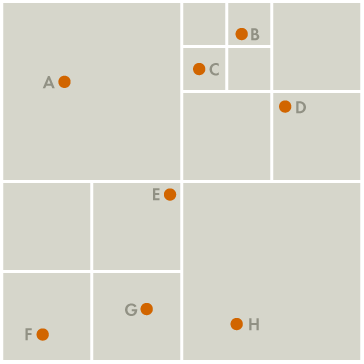
\includegraphics[width=0.65\linewidth]{Images/bh1.png}}
                  {http://arborjs.org/docs/img/example-space.png}
\end{figure}
\end{frame}

\begin{frame}
\begin{figure}
\centering
\includegraphics[width=0.9\linewidth]{Images/Barnes–Hut check_1000.png}
\end{figure}
\end{frame}


\subsection{Milky Way Potential}

\begin{frame}

Multi-component axis-symmetric potential

\begin{itemize}
\item components
\begin{itemize}
\item Black hole: Keplerian potential
\item Disk: Miyamoto Nagai potential
\item Bulge: Hernquist potential
\item Dark matter halo: Navarro–Frenk–White potential
\end{itemize}
\item needed for

\begin{itemize}
\item Force from analytic derivatives
\item Initial conditions for field stars
\end{itemize}
\end{itemize}


\end{frame}








\end{document}